\documentclass[10.5pt,scale=1.0,t,aspectratio=169,hyperref={pdfpagelabels=false}]{beamer}
%\usepackage[paperwidth=13.33in, paperheight=7.5in,top=.25in, bottom=.25in, left=.25in, right=.25in]{geometry}
%\geometry{papersize={13.33in,7.5in}}

%\usetheme{Dresden}
%\usetheme{Warsaw}

%Other themes
%https://hartwork.org/beamer-theme-matrix/

\usepackage{lipsum}
\usepackage{color}

\usepackage{amsfonts}
\usepackage{amsmath,mathtools}
\usepackage{mathrsfs}
\usepackage{array}
\usepackage{algorithm}
\usepackage{hyperref}
\usepackage[spanish,es-nodecimaldot]{babel}
\usepackage[utf8]{inputenc}
%\usepackage{intcalc}
\usepackage{graphicx}
\usepackage{multicol}
%\usepackage{authblk}
\usepackage{multirow}
\usepackage{enumitem}
\usepackage[document]{ragged2e}

\usepackage[absolute,overlay]{textpos}
\textblockorigin{0mm}{0mm} 

\usefonttheme[onlymath]{serif}
%\usepackage{epstopdf}
\usepackage{verbatim}
\usepackage{cite}
%\usepackage[texcoord,grid,gridunit=mm,gridcolor=red!10,subgridcolor=green!10]{eso-pic}




\newenvironment{conditions}[1][where:]
{#1 \begin{tabular}[t]{>{$}l<{$} @{${}={}$} l}}
	{\end{tabular}\\[\belowdisplayskip]}


\newcolumntype{L}{>{$}l<{$}} % math-mode version of "l" column type


\newcounter{saveenumi}
\newcommand{\seti}{\setcounter{saveenumi}{\value{enumi}}}
\newcommand{\conti}{\setcounter{enumi}{\value{saveenumi}}}

\setbeamertemplate{bibliography item}{\insertbiblabel}


\hypersetup{colorlinks=true,
	linkcolor=blue,
	linktoc=all,				
	citecolor=blue,
	urlcolor=red,
	pdftitle={ELECTRONICA DIGITAL},
	pdfauthor={Santiago Rúa Pérez},
	pdfcreator={Santiago Rúa Pérez}}


\definecolor{GreenDark}{rgb}{0.0, 0.60, 0.0}
\definecolor{RedDark}{rgb}{183, 0.0, 0.0}
\definecolor{BlueDark}{rgb}{0.0, 0.0, 167}
\definecolor{BlueLight}{rgb}{0.2, 0.451, 0.517}


\graphicspath{{imag/}}

\newcommand{\Ho}{$H_{0}$}
\newcommand{\Ha}{$H_{a}$}
\newcommand{\Nota}{{\bf Nota: }}
\newcolumntype{P}[1]{>{\centering\arraybackslash}p{#1}}
\newcolumntype{M}[1]{>{\centering\arraybackslash}m{#1}}

\newcommand{\less}{<}
\newcommand{\greater}{>}


\setlength{\parindent}{1em}
\setlength{\parskip}{.6em}
\renewcommand{\baselinestretch}{.9}

%%%%    C environment    ---------------- %%%%%%%%%%%%%%%.
\usepackage{listings}
\usepackage{xcolor}
\definecolor{mGreen}{rgb}{0,0.6,0}
\definecolor{mGray}{rgb}{0.5,0.5,0.5}
\definecolor{mPurple}{rgb}{0.58,0,0.82}
\definecolor{backgroundColour}{rgb}{0.95,0.95,0.92}

\lstdefinestyle{CStyle}{
	backgroundcolor=\color{backgroundColour},   
	commentstyle=\color{mGreen},
	keywordstyle=\color{magenta},
	numberstyle=\tiny\color{mGray},
	stringstyle=\color{mPurple},
	basicstyle=\tiny,
	breakatwhitespace=false,         
	breaklines=true,                 
	captionpos=b,                    
	keepspaces=true,                 
	numbers=left,                    
	numbersep=5pt,                  
	showspaces=false,                
	showstringspaces=false,
	showtabs=false,                  
	tabsize=2,
	language=C
}
%%--------------------------------------------------------------------------


\title{Electrónica digital II}   
\author{Santiago Rúa Pérez, PhD.} 
\date{\today} 

\setlength{\TPHorizModule}{\textwidth}
\setlength{\TPVertModule}{\textwidth}

\newcommand{\btVFill}{\vskip0pt plus 1filll}


\setbeamertemplate{sidebar right}{}
\setbeamertemplate{footline}
{
	\leavevmode%
	\hbox{%
		\begin{beamercolorbox}[wd=.333333\paperwidth,ht=2.25ex,dp=1ex,center]{author in head/foot}%
			\usebeamerfont{author in head/foot}\insertshortauthor
		\end{beamercolorbox}%
		\begin{beamercolorbox}[wd=.333333\paperwidth,ht=2.25ex,dp=1ex,center]{title in head/foot}%
			\usebeamerfont{title in head/foot}\insertshorttitle
	\end{beamercolorbox}}%
	\vskip0pt%
}
\makeatother

\begin{document}
	%%%%%%%%%%%%%%%%%% FRAME %%%%%%%%%%%%%%%%%%%%%%%%%%
	\begin{frame}
		\titlepage
	\end{frame}
	%%%%%%%%%%%%%%%%% FRAME START %%%%%%%%%%%%%%%%%%%%%%%%%%
	\frame{
		%\frametitle{}
		\begin{center}
			\LARGE \textcolor{blue}{FUNCIONES Y LIBRERIAS EN C}
		\end{center}
		
	}
	%%%%%%%%%%%%%%%%% FRAME START %%%%%%%%%%%%%%%%%%%%%%%%%%
%%%%%%%%%%%%%%%%% FRAME START %%%%%%%%%%%%%%%%%%%%%%%%%%

%%%%%%%%%%%%%%%%% FRAME %%%%%%%%%%%%%%%%%%%%%%%%%%
\begin{frame}
	\frametitle{Programaci\'on modular}
	{\bf Objetivos}
	\begin{itemize}
	\item Construir programas modulares.
	\item Usar funciones de la libreria math.
	\item Pasar información entre funciones.
	\item Recursividad.
	\end{itemize}
\end{frame}
%%%%%%%%%%%%%%%%% FRAME %%%%%%%%%%%%%%%%%%%%%%%%%%
\begin{frame}
\frametitle{Modularizar programas en C}
	En C, las funciones son utilizadas para modularizar programas. El objetivo es empaquetar pedazos de código para luego reutilizarlo.
	\begin{figure}
		\centering
		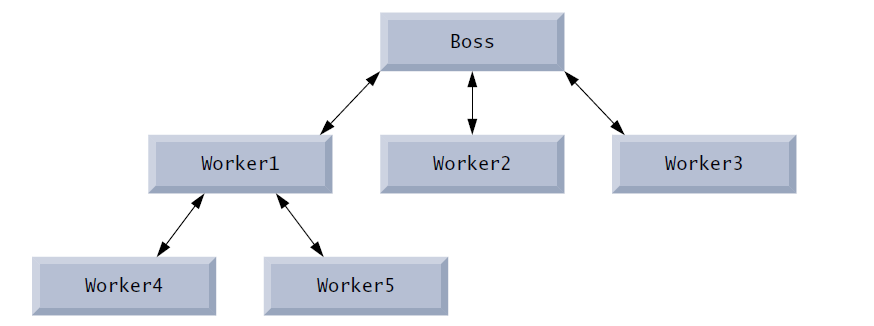
\includegraphics[width=10cm]{FuncionesModularidad}
	\end{figure}
\end{frame}

%%%%%%%%%%%%%%%%% FRAME %%%%%%%%%%%%%%%%%%%%%%%%%%
\begin{frame}
	\frametitle{Funciones de la libreria math.h}
	Esta libreria posibilita realizar operaciones matemáticas especializadas.
	\begin{figure}
		\centering
		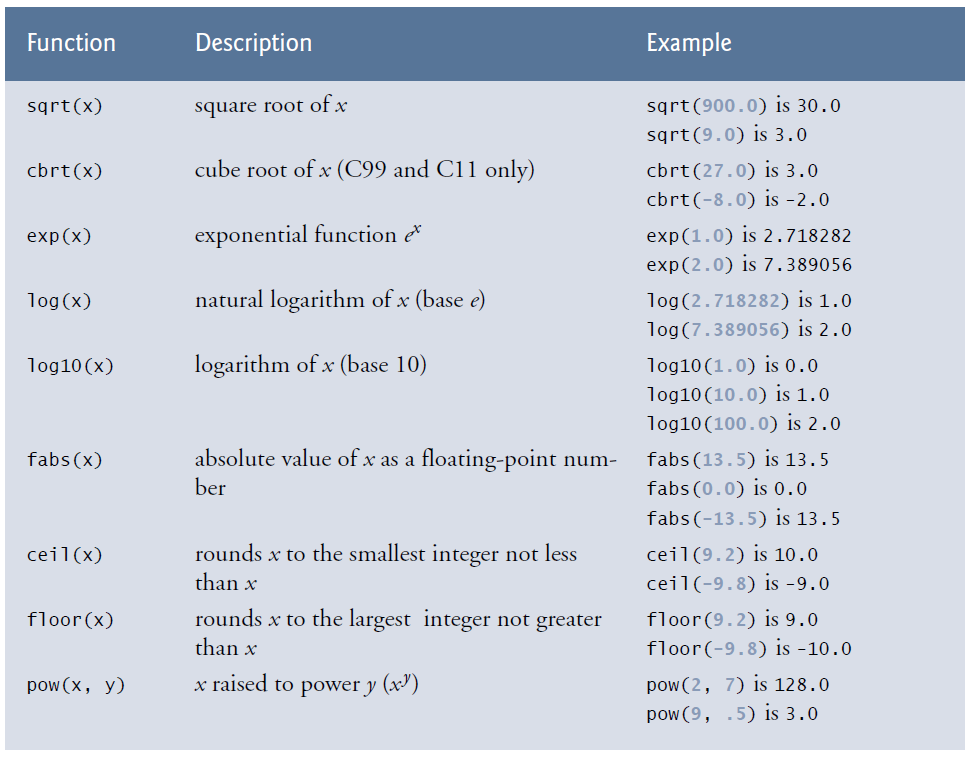
\includegraphics[width=8cm]{MathLibrary}
	\end{figure}
	
\end{frame}

%%%%%%%%%%%%%%%%% FRAME %%%%%%%%%%%%%%%%%%%%%%%%%%
\begin{frame}[fragile]
	\frametitle{Definición de una función}
	El objetivo de las funciones consiste en modularizar un software. Todas las variables definidas dentro de la función son locales. Las funciones deben crearse con proptotipo y la ejecución.
	\begin{lstlisting}[style=CStyle]
		#include <stdio.h>
		
		int square(int y); // function prototype
		
		int main(void)
		{
			// loop 10 times and calculate and output square of x each time
			for (int x = 1; x <= 10; ++x) {
				printf("% d ",square(x)); // function call
			}
			puts("");
		}
		
		int square(int y) // y is a copy of the argument to the function
		{
			return y * y; // returns the square of y as an int
		}
	\end{lstlisting}
	\textbf{Ejemplo}: realizar una funcion que reciba tres numeros enteros y retorne cual es el mayor. 
\end{frame}

%%%%%%%%%%%%%%%%% FRAME %%%%%%%%%%%%%%%%%%%%%%%%%%
\begin{frame}[fragile]
	\frametitle{Solucion Ejemplo}
	\begin{lstlisting}[style=CStyle]
		#include <stdio.h>
		
		int maximum(int x,int y, int z);
		
		int main (void){
			int number1; // first integer entered by the user
			int number2; // second integer entered by the user
			int number3; // third integer entered by the user
			
			printf("% s", "Enter three integers: ");
			scanf("% d% d% d", &number1, &number2, &number3);
			
			// number1, number2 and number3 are arguments
			// to the maximum function call
			printf("El numero maximo es: % d\n", maximum(number1,number2,number3));
		}
		
		// Definicion de la funcion
		// x, y and z are parameters
		int maximum(int x, int y, int z)
		{
			int max = x; // assume x is largest
			if (y > max) { // if y is larger than max,
				max = y; // assign y to max
			}
			if (z > max) { // if z is larger than max,
				max = z; // assign z to max
			}
			return max;
		}
	\end{lstlisting}
\end{frame}

%%%%%%%%%%%%%%%%% FRAME %%%%%%%%%%%%%%%%%%%%%%%%%%
\begin{frame}[fragile]
	\frametitle{Pila llamadas a funciones}
	Es importante entender el concepto de una pila. Las pilas funcionan como el último dato que entra a la pila es el primero en salir. En cada llamado de función se debe almacenar el contexto donde se está trabajando y la dirección de memoria de donde fue llamado. Supongamos que se tiene el siguiente código.
	
	\begin{lstlisting}[style=CStyle]
		#include <stdio.h>
		
		int square(int y); // function prototype
		
		int main(void)
		{
			int a = 10; // value to square (local automatic variable in main)
			
			printf("%d squared: %d\n", square(a) ); // display a squared
		}
		
		int square(int y) // y is a copy of the argument to the function
		{
			return y * y; // returns the square of y as an int
		}
	\end{lstlisting}
\end{frame}

%%%%%%%%%%%%%%%%% FRAME %%%%%%%%%%%%%%%%%%%%%%%%%%
\begin{frame}
	\frametitle{Pila llamadas a funciones}
	\begin{columns}
		\column{0.5\linewidth}
		\begin{figure}
			\centering
			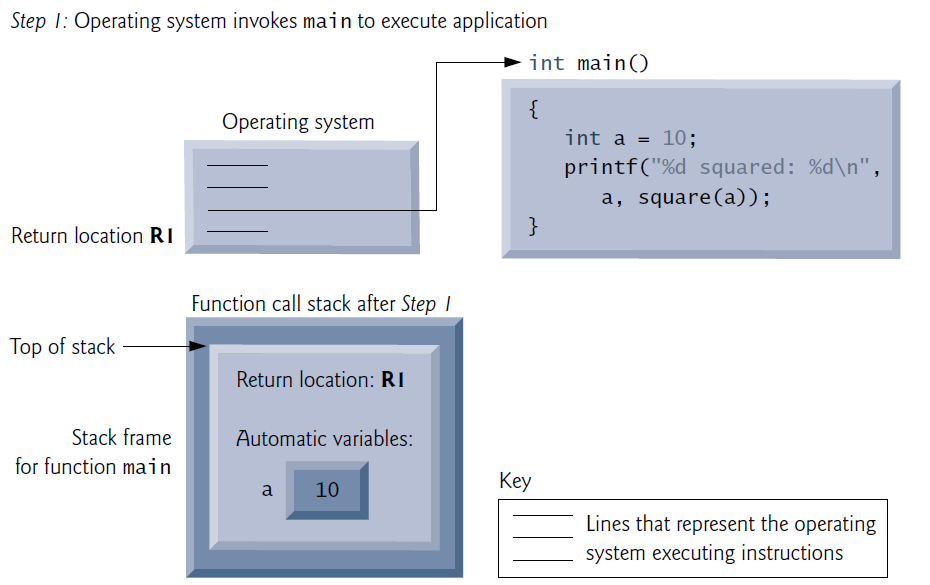
\includegraphics[scale=0.45]{Stack1}
		\end{figure}
	
		\column{0.5\linewidth}
		\begin{figure}
			\centering
			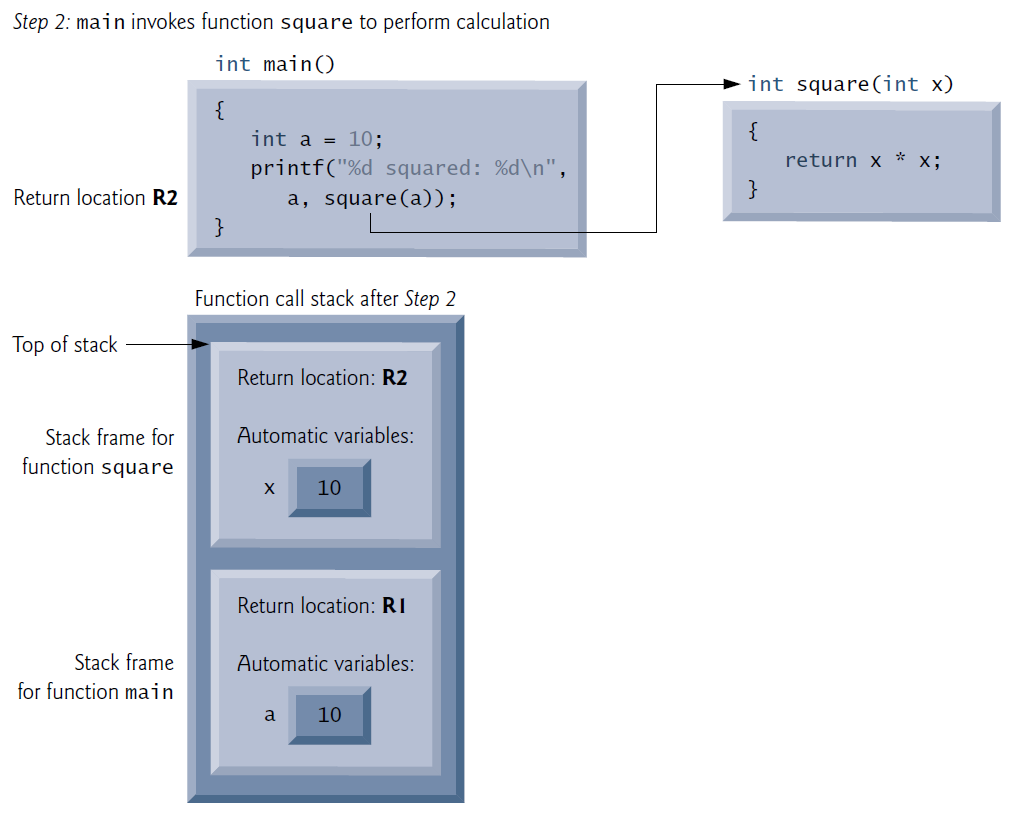
\includegraphics[scale=0.43]{Stack2}
		\end{figure}
	\end{columns}
\end{frame}

%%%%%%%%%%%%%%%%% FRAME %%%%%%%%%%%%%%%%%%%%%%%%%%
\begin{frame}
	\frametitle{Pila llamadas a funciones}
	\begin{columns}
		\column{0.5\linewidth}
		\begin{figure}
			\centering
			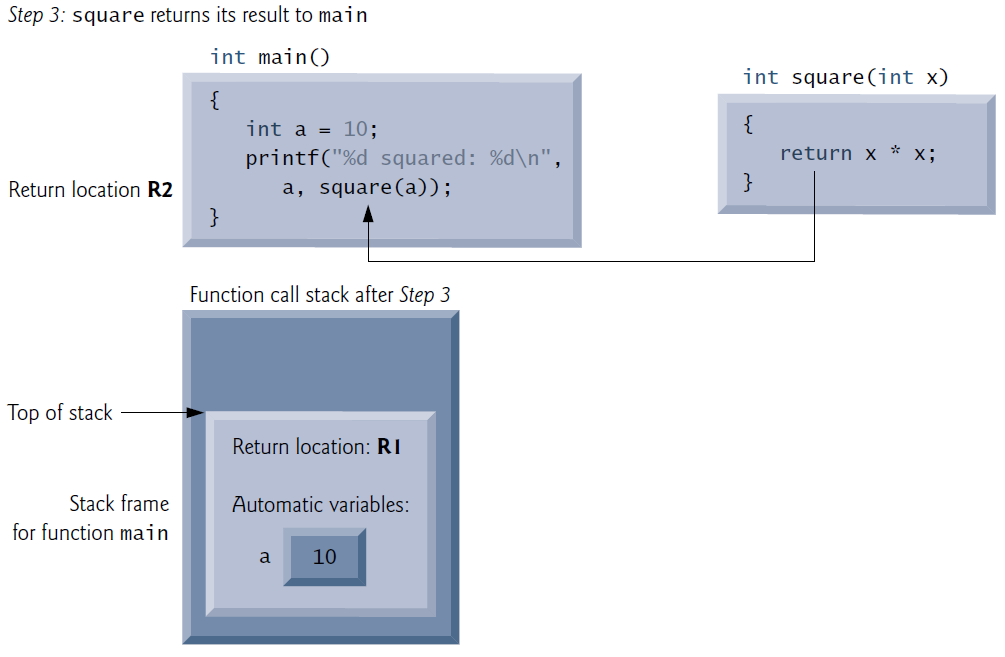
\includegraphics[scale=0.45]{Stack3}
		\end{figure}
		
		\column{0.5\linewidth}
		
	\end{columns}
\end{frame}

%%%%%%%%%%%%%%%%% FRAME %%%%%%%%%%%%%%%%%%%%%%%%%%
\begin{frame}
	\frametitle{Scanf y Printf}
	\begin{figure}
		\centering
		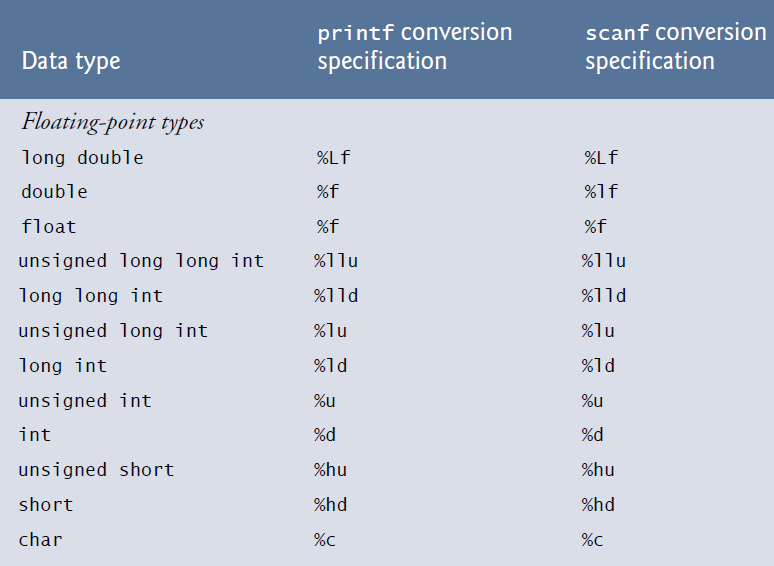
\includegraphics[width=8cm]{PrintfScanf}
	\end{figure}
	
\end{frame}
%%%%%%%%%%%%%%%%% FRAME %%%%%%%%%%%%%%%%%%%%%%%%%%
\begin{frame}
	\frametitle{Headers}
	Cada libreria contiene un header. Estos header contienen los prototipos de las funciones en la libreria y las definiciones de varios tipos de datos. 
	\begin{figure}
		\centering
		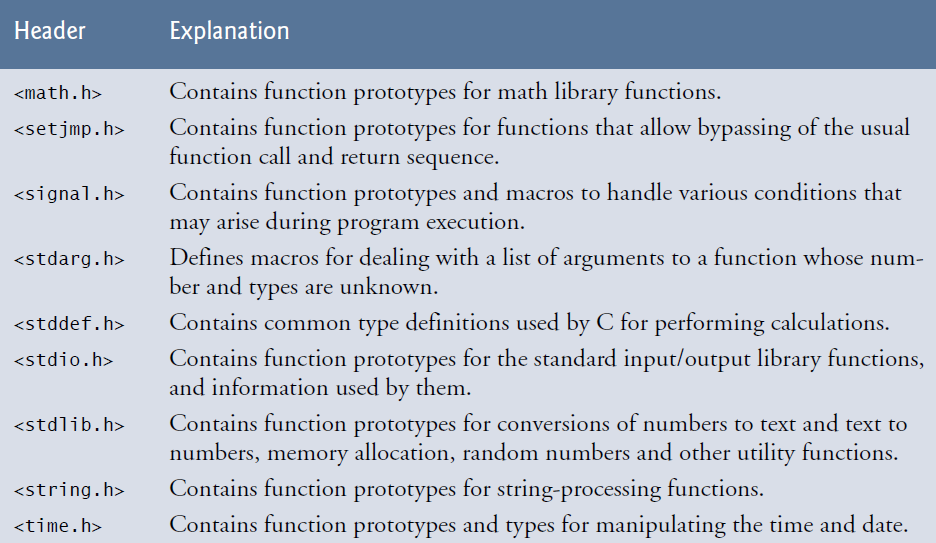
\includegraphics[width=8cm]{Headers}
	\end{figure}
	Las comillas dobles para librerias propias.
\end{frame}
%%%%%%%%%%%%%%%%% FRAME %%%%%%%%%%%%%%%%%%%%%%%%%%
\begin{frame}
	\frametitle{Random Number Generation}
	La función rand() se encuentra en la libreria stdlib.h. Esta función generar un entero entre 0 y \texttt{RAND\_MAX} el cual por defecto es 32767.
	
	\textbf{Ejemplo}: Hacer un programa que simule lanzar los dados 20 veces e imprima su valor.
	
	Las función rand() arroja número pseudoaleatorios. Para generar número aleatorios reales es importante usar la funcion srand(seed) para indicar la semilla a usar.
\end{frame}
%%%%%%%%%%%%%%%%% FRAME %%%%%%%%%%%%%%%%%%%%%%%%%%
\begin{frame}[fragile]
	\frametitle{Random Number Generation - Solución}
	\begin{lstlisting}[style=CStyle]
		#include <stdio.h>
		#include <stdlib.h>
		
		int main(void)
		{
			// loop 20 times
			for (unsigned int i = 1; i <= 20; ++i) {
				
				// pick random number from 1 to 6 and output it
				printf("%10d", 1 + (rand() % 6));
				
				// if counter is divisible by 5, begin new line of output
				if (i % 5 == 0) {
					puts("");
				}
			}
		}
	\end{lstlisting}
\end{frame}
%%%%%%%%%%%%%%%%% FRAME %%%%%%%%%%%%%%%%%%%%%%%%%%
\begin{frame}
	\frametitle{Random Number Generation - Ejemplo 2}
	\textbf{Ejemplo}: Un jugador lanza el dado dos veces. Despues de lanzarlos realiza la suma de ambos dados. Si la suma es 7 u 11 en el primer lanzamiento, entonces el jugador gana. Si es 2, 3, o 12 entonces pierde. Si la suma es 4, 5, 6, 8, 9, o 10, entonces esa suma se convierte en el punto del jugador. Para ganar debe continuar lanzando los dados hasta que hagas el puntaje. El jugador pierde si lanza una suma de 7.
	
	\textbf{Hint}: Haga una funcion que haga el lanzamiento de los dados y retorne la suma. 
	
	\textbf{Hint 2}: utilice enum para crear los posibles casos: \texttt{enum Status \{ CONTINUE, WON, LOST \};}
\end{frame}
%%%%%%%%%%%%%%%%% FRAME %%%%%%%%%%%%%%%%%%%%%%%%%%
\begin{frame}[fragile]
	\frametitle{Random Number Generation - Solución}
	\begin{lstlisting}[style=CStyle]
	#include <stdio.h>
	#include <stdlib.h>
	#include <time.h> // contains prototype for function time
	
	// enumeration constants represent game status
	enum Status { CONTINUE, WON, LOST };
	
	int rollDice(void); // function prototype
	
	int main(void)
	{
		// randomize random number generator using current time
		srand(time(NULL));
		
		int myPoint; // player must make this point to win
		enum Status gameStatus;// can contain CONTINUE, WON, or LOST
		int sum = rollDice(); // first roll of the dice
		
		switch(sum) {
			case 7: case 11: // 7 and 11 is a winner
			gameStatus = WON;
			break;
			case 2:  case 3: case 12:// 2, 3 and 12 is a loser
			gameStatus = LOST;
			break;
			default:
			gameStatus = CONTINUE; // player should keep rolling
			myPoint = sum; // remember the point
			printf("Point is % d\n", myPoint);
			break; // optional
		}
	\end{lstlisting}
\end{frame}
%%%%%%%%%%%%%%%%% FRAME %%%%%%%%%%%%%%%%%%%%%%%%%%
\begin{frame}[fragile]
	\frametitle{Random Number Generation - Solución}
	\begin{lstlisting}[style=CStyle]
		    while (CONTINUE == gameStatus) { // player should keep rolling
				sum = rollDice(); // roll dice again
				if (sum == myPoint) { // win by making point
					gameStatus = WON;
				}
				else {
					if (7 == sum) { // lose by rolling 7
						gameStatus = LOST;
					}
				}
			}
			if (WON == gameStatus) { // did player win?
				puts("Player wins");
			}
			else { // player lost
				puts("Player loses");
			}
		}
		
		int rollDice(void){
			int die1 = 1 + (rand() % 6); // pick random die1 value
			int die2 = 1 + (rand() % 6); // pick random die2 value
			
			printf("Player rolled % d + % d = % d\n", die1, die2, die1 + die2);
			return die1 + die2; // return sum of dice
		}
		\end{lstlisting}
	\end{frame}
%%%%%%%%%%%%%%%%% FRAME %%%%%%%%%%%%%%%%%%%%%%%%%%
\begin{frame}
	\frametitle{Variables Locales vs Globales}
	Todas las variables definidas dentro de una función estan solo al alcance de esa función y se conocen como variables locales. Por otro lado las variables globales tienen alcance a todos. Cuando se le pone el prefijo de estático conserva su valor en el tiempo. 
	\begin{figure}
		\centering
		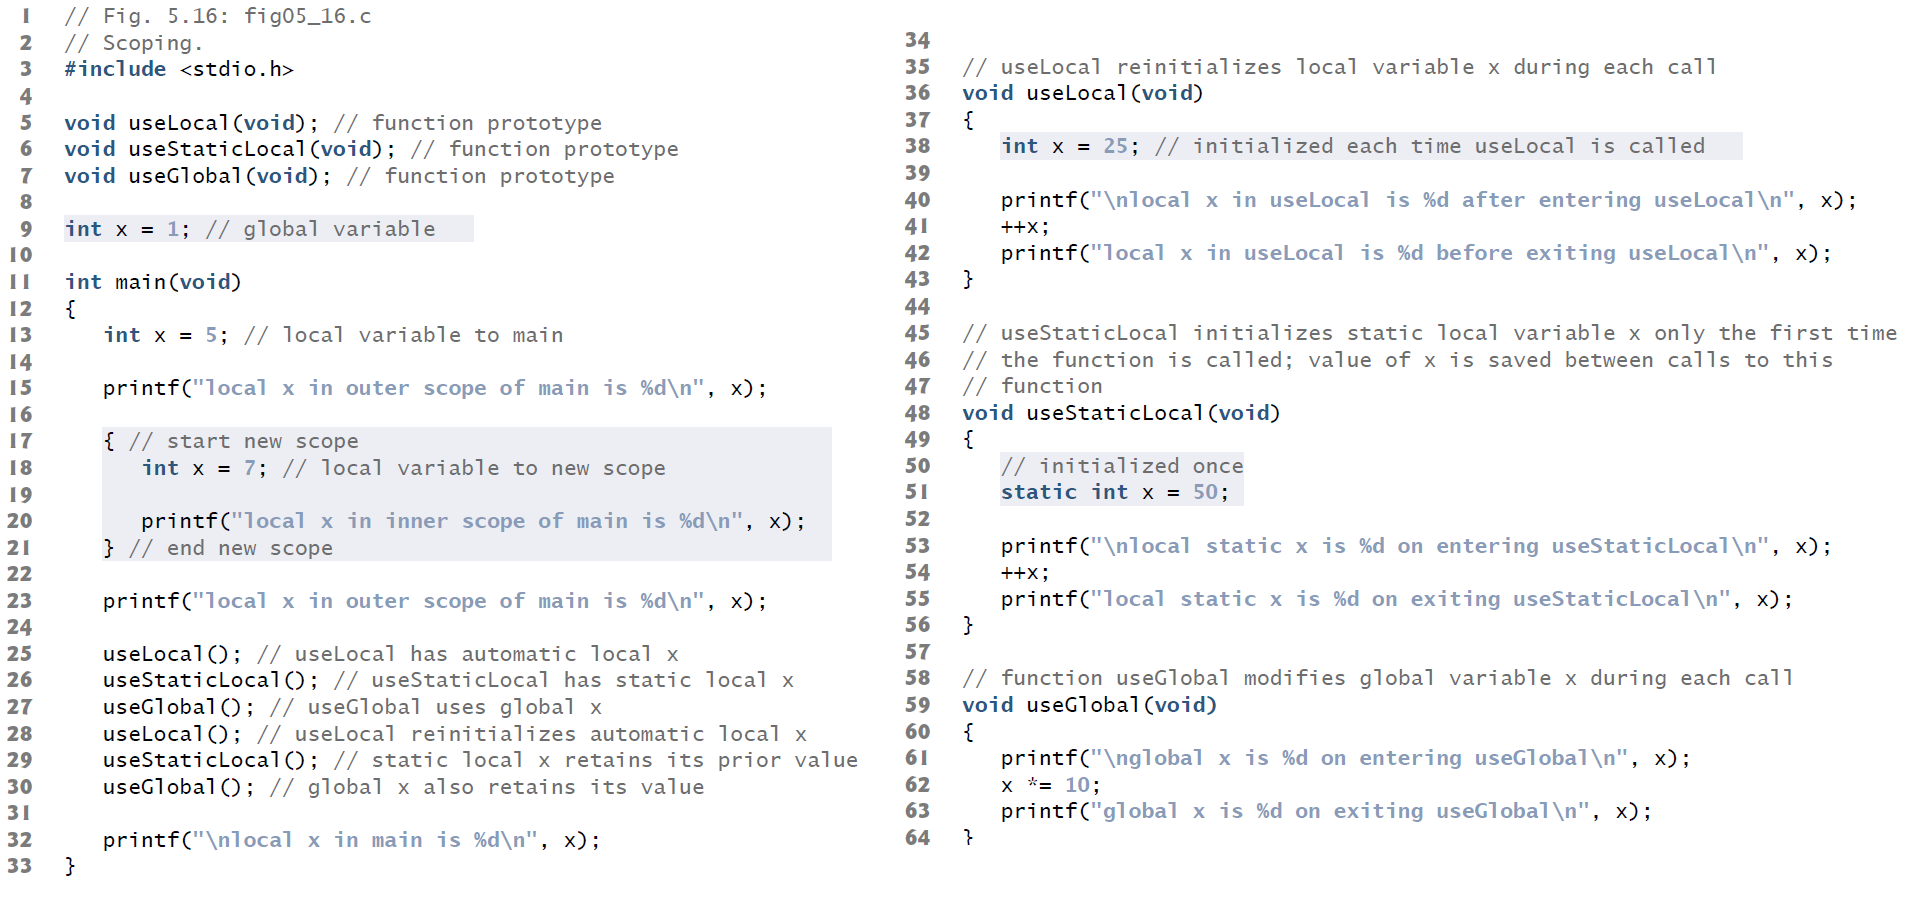
\includegraphics[width=10cm]{GlobalLocal}
	\end{figure}
\end{frame}

%%%%%%%%%%%%%%%%% FRAME %%%%%%%%%%%%%%%%%%%%%%%%%%
\begin{frame}[fragile]
	\frametitle{Librerias propias}
	El objetivo de las librerias propias en modularizar el programa con funciones y archivos creados por nosotros mismos. Independizar estas funciones del código generan mayor modularidad.
	{\footnotesize
	\begin{itemize}
		\item Cada libreria tiene dos archivos: un .h o header de las funciones, y un .c donde esta definida la función. 
		\item El archivo .h debe comenzar indicandole al procesador el procedimiento a compilar. Es decir:
		\begin{lstlisting}[style=CStyle]
			#ifndef _LIBRERIAPROPIA
			#define _LIBRERIAPROPIA
			
			// ---- Variables globales y definiciones ------//
			
			// ---- Prototipos de funciones --------//
			
			...
			...
			
			#endif
		\end{lstlisting}
		\item El archivo .c debe hacer un llamado a su propio header donde estan los prototipos e incluir librerias propias del sistema operativo necesarias. 
		\item Posteriormente pueden ser llamadas desde el programa principal.
	\end{itemize}
	}
	\textbf{Ejemplo}: Crear una libreria propia con dos o tres funciones de las antes creadas. Compilar usar \href{https://www.cs.colby.edu/maxwell/courses/tutorials/maketutor/}{Makefile}
\end{frame}
%%%%%%%%%%%%%%%%% FRAME %%%%%%%%%%%%%%%%%%%%%%%%%%
\begin{frame}
	\frametitle{Recursividad}
	Consiste en llamarse asi mismo. Una función recursiva es aquella que tiene un llamado a si misma. \textbf{Ejemplo}: factorial.
	\begin{figure}
		\centering
		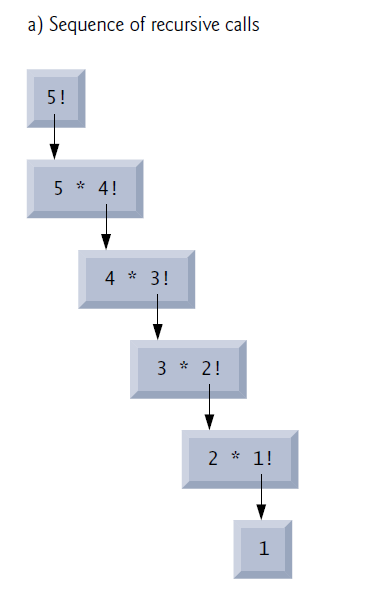
\includegraphics[scale=0.5]{Factorial}
	\end{figure}
	Como implementarlo? 
\end{frame}

%%%%%%%%%%%%%%%%% FRAME %%%%%%%%%%%%%%%%%%%%%%%%%%
\begin{frame}[fragile]
	\frametitle{Factorial - Soluci\'on}
		\begin{lstlisting}[style=CStyle]
			#include <stdio.h>
			
			unsigned long long int factorial(unsigned int number);
			
			int main(void)
			{
				// during each iteration, calculate
				// factorial(i) and display result
				for (unsigned int i = 0; i <= 21; ++i) {
					printf("% u! = % llu\n", i, factorial(i));
				}
			}
			
			// recursive definition of function factorial
			unsigned long long int factorial(unsigned int number)
			{
				// base case
				if (number <= 1) {
					return 1;
				}
				else { // recursive step
					return (number * factorial(number - 1));
				}
			}
		\end{lstlisting}
	\textbf{Tarea}: implementar la serie de Fibonnaci.
\end{frame}
%%%%%%%%%%%%%%%%%% FRAME %%%%%%%%%%%%%%%%%%%%%%%%%%
%\frame{
%	\frametitle{Arreglos}
%	Es un conjunto de datos organizados de forma contigua en memoria.  
%	\begin{figure}
%		\centering
%		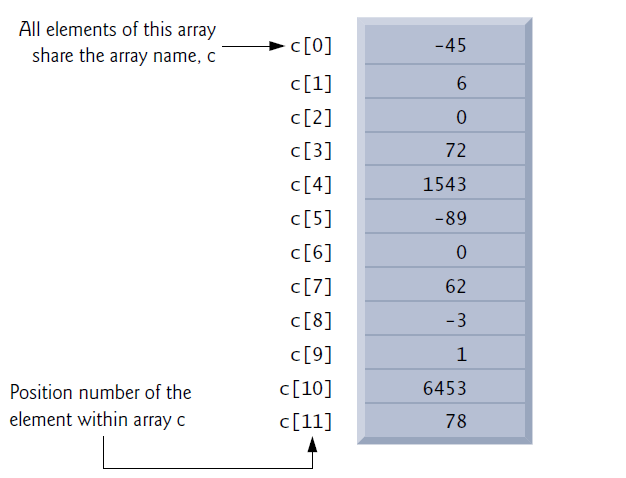
\includegraphics[scale=0.5]{Array}
%	\end{figure}
%}
%%%%%%%%%%%%%%%%%% FRAME %%%%%%%%%%%%%%%%%%%%%%%%%%
%\frame{
%	\frametitle{Arreglos - Declaración}
%	Para crear un vector basta con indicar el nombre del vector y el tamaño del mismo, de esta forma se le da la orden al compilador el espacio en memoria. 
%	\begin{figure}
%		\centering
%		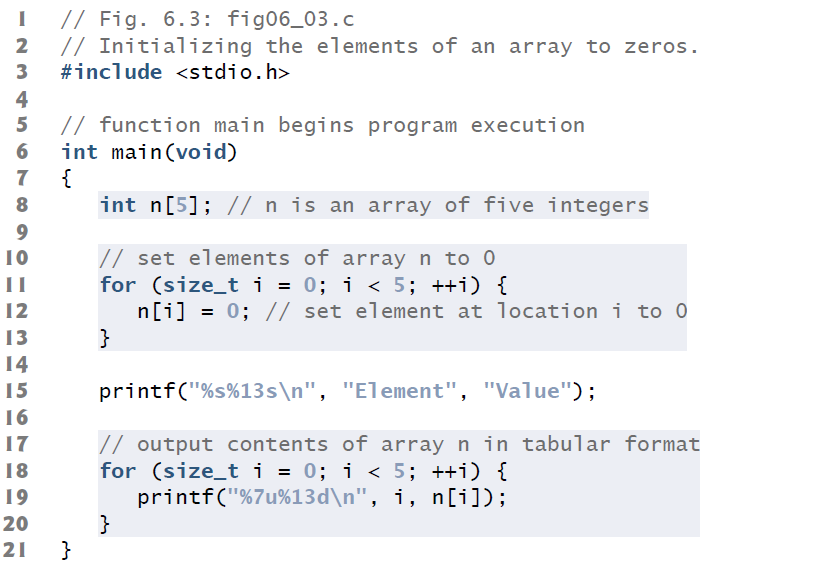
\includegraphics[scale=0.5]{EjemploArray}
%	\end{figure}
%	Pueden inicializarse mediante lista de elementos. También se puede definir la directiva de preprocesamiento \texttt{\#define}. 
%}
%%%%%%%%%%%%%%%%%% FRAME %%%%%%%%%%%%%%%%%%%%%%%%%%
%\frame{
%	\frametitle{Arreglos - Ejercicio}
%	\begin{itemize}
%		\item 	Cuarenta estudiantes fueron encuestados sobre la calidad de comida en un restaurante es un escala de 1 a 10 siendo está última como la mejor. Ponga las 40 respuestas en un vector de enteros y encuentre el resumen de los resultados de la encuesta. 
%		\item Lance los dados 60000000 de veces y haga un resumen de los resultados.  
%		\item Haga un programa que dado un vector de tamaño n, los organice de mayor a menor. 
%	\end{itemize} 
%}
%%%%%%%%%%%%%%%%%% FRAME %%%%%%%%%%%%%%%%%%%%%%%%%%
%\frame{
%	\frametitle{Arreglos - Multidimensionales}
%	Un arreglo multidimensional consiste en formar un vector de vectores. 
%	\begin{figure}
%		\centering
%		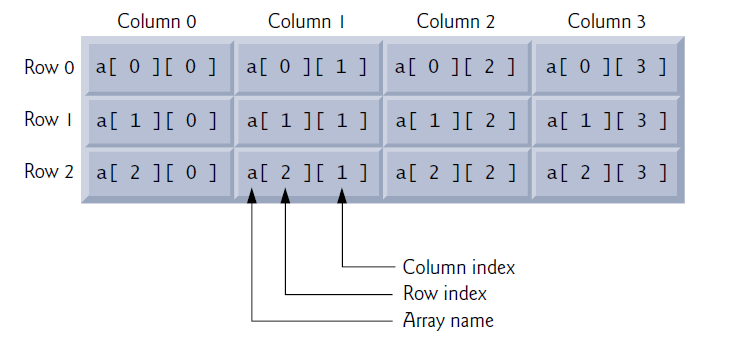
\includegraphics[scale=0.5]{Matriz}
%	\end{figure}
%}
%%%%%%%%%%%%%%%%%% FRAME %%%%%%%%%%%%%%%%%%%%%%%%%%
%\frame{
%	\frametitle{Arreglos - Multidimensionales - Ejemplo}
%	\begin{figure}
%		\centering
%		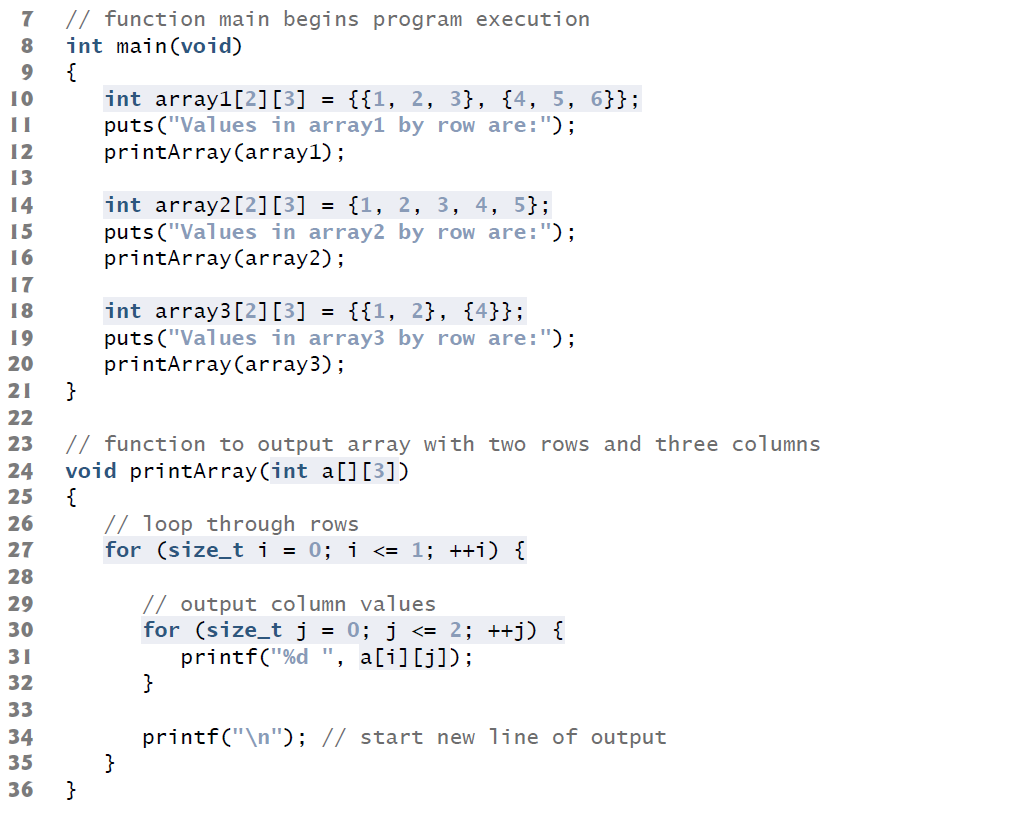
\includegraphics[scale=0.5]{EjemploMatriz}
%	\end{figure}
%}
%%%%%%%%%%%%%%%%%% FRAME %%%%%%%%%%%%%%%%%%%%%%%%%%
%\frame{
%	\frametitle{Arreglos - Multidimensionales - Ejemplo}
%	Implemente un programa que dado una matriz de notas de estudiantes, obtenga la menor nota, la mayor nota, y el promedio de cada estudiante. 
%	
%	\begin{figure}
%		\centering
%		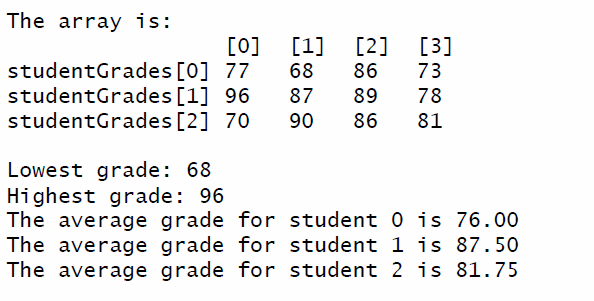
\includegraphics[scale=0.5]{EjemploNotas}
%	\end{figure}
%}
%%%%%%%%%%%%%%%%% FRAME %%%%%%%%%%%%%%%%%%%%%%%%%%
\frame{
\begin{center}
	\LARGE \textcolor{blue}{FUNCIONES Y LIBRERIAS EN C}
\end{center}

\begin{center}
	\LARGE \textcolor{blue}{GRACIAS}
\end{center}
}

%%%%%%%%%%%%%%%%%%%%%%%%%%%%%%%%%%%%%%%%%%%%%%%%%%%%%%%%%%%%%%%%%%%%%%%%%%%%%%%%%%%%%%%%%%%%%%%%%%%%%%%%%%%%%



\end{document}

